\documentclass[10pt]{article}
\usepackage[margin=0.65in]{geometry}
\usepackage[T1]{fontenc}
\usepackage{lmodern,graphicx,booktabs,hyperref}
\setlength{\parindent}{0pt}\setlength{\parskip}{5pt}\setlength{\emergencystretch}{3em}
\begin{document}
{\Large\bfseries Warmup-only CPU preflight: complete recovery and control repairs}

23 November 2026; phase 05, 13:37:24--13:39:07 UTC. Unsigned producer record
\texttt{PCC-20261123-a79757}; authenticated execution standing is not established.

All \textbf{36 of 36 calls on 12 distinct public targets} complete, with per-target
full certificate bytes and structural counters equal across parent/candidate/A-A.
All external Native replays and all required OpenSSL controls pass. These are
warmups; none is a main-panel sample.

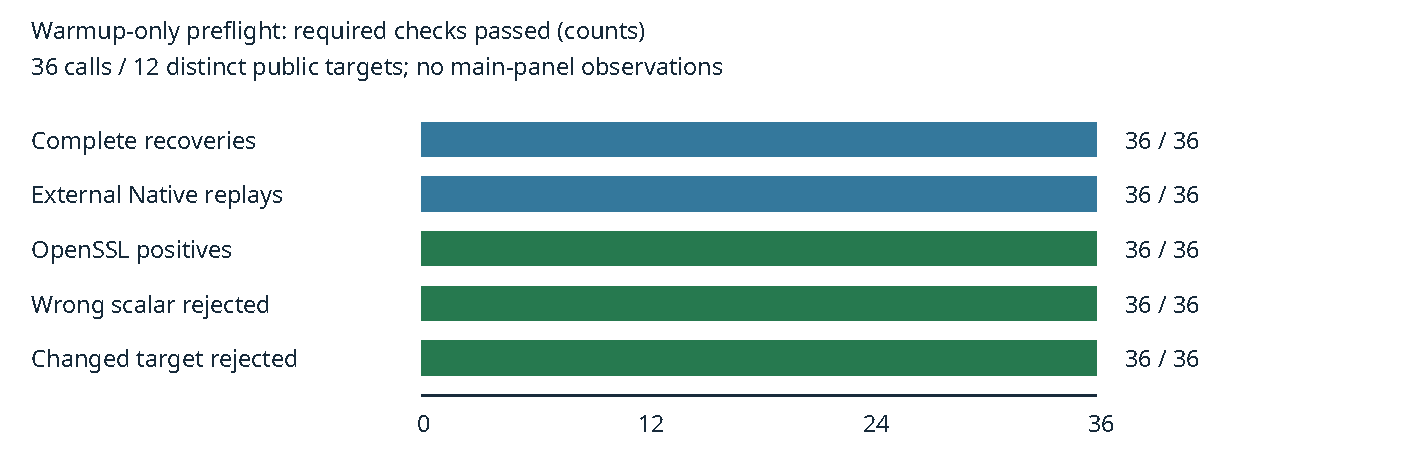
\includegraphics[width=\linewidth]{coverage.pdf}

\textbf{Inputs and custody.} Same six prime-field fixtures 20/24/28/32/36/40 bits,
order bits 20/25/28/32/36/41, seeds 101/202, m8/batch64. Public x-search target
construction supplies no scalar. Two 108-input worker snapshots differ only in
the exact staged/reverse-pass numerator library; 47 checks pass per source.
Published preparation 04307332 precedes data. All 239 post-call input/binary hashes
match. Separate output directories preserve native u, replicate 0 and warmup false fields.

\textbf{Local conditions.} One worker, no concurrent builds/tests,worker/external
Native affinity CPU 4. 120s worker/60s replay, 300s whole preflight, one attempt/no
retries. Worker-only 4GiB virtual limit; sampled whole-cgroup peak 13,817,049,088 bytes
includes retained other research, not per-process RSS. No physical stop.
103s coarse wall span gives 104 x 10 x 1.25 = 1300s conservative main planning estimate,
not a guarantee. Clocks are L0; CPU time, total-operation S and peak RSS unmeasured.

\textbf{Verification scope.} OpenSSL reconstructs the fixed public target and
checks nonidentity,\texttt{rP=O},\texttt{kP=Q} using separate point arithmetic.
Wrong scalars reject at scalar equality; consistent \texttt{(r-k,-Q)} substitutions
reject at public-target binding. It does not independently establish prime/Hasse
admission, full relations or execution history. Native full replay shares solver
arithmetic. The 12 targets are repeated across 3 arms, not 36 independent instances.

\textbf{Prospective repairs.} Review 11 retains real original gaps: nested process
groups, failure-path finalization/clock checking, launcher pinning and per-target
order imbalance. Separate V2 code adds balanced 9-round positions,clock/exit
validation and foreground timeouts; supervisor always attempts separate
finalization after terminal. Ten controls pass. A mock failure retains incomplete
flow; a group-TERM control leaves no live recorded owned process (some zombies).
It does not stress RAM threshold or virtual-limit enforcement.

\textbf{Source binding and dry analysis.} A later 15-input source-prehashed clean
build reproduces all 4 earlier V2 binaries byte-for-byte, then copied qualification
passes with source/binary pins. Original pre-unit custody gaps stay recorded.
Valid preflight analysis/CSV/SVG reproduce exactly. A synthetic fixture copies
36 warmups into 360 metadata cells solely to test 36 nine-value summaries; 0 new solver
or timing observations. It is excluded from main data.

\textbf{Next boundary.} Main 360 calls remain unstarted at this snapshot:
36 warmups/324 measured, 12 targets. Freeze/publish/read back exact source, host, config,
protocol and launchers first. 1500/120/120s enforced phases plus grace are a nominal
1800s planning envelope,not an overall watchdog. Local, classical, no S3 or extra
cloud spend. Prior 24-call/round24/round25/84-case records remain unchanged.

\small Sources: \path{PREFLIGHT-OUTCOME.md},\path{MAIN-PROTOCOL.md},reviews 10--12;
raw records \path{/tmp/ecdlp-cpu-comparison-20261123/preflight}. Native analysis
and point-audit summary supply the exact plotted counts; no uncertainty interval
is needed for this recorded census.\par
\url{https://github.com/isogeny-labs/crypto/pull/4996}
\end{document}
